\subsection{Partial SPIDER}

The \textit{SPIDER} algorithm \cite{bauckmann2006efficiently} was developed for unary IND discovery. \textit{SPIDER} executes a sort merge join across all columns. It functions in two primary stages. First, it sorts each attribute and saves the sorted data in separate files for each attribute. Then, it performs a $k$-way merge while simultaneously verifying the candidates.

To extend the \textit{SPIDER} algorithm for pIND discovery, we need to monitor the frequency of each value alongside the total count of unique values. Bauckmann et al. have already proposed an adjusted algorithm capable of pIND discovery. Their suggestion involves integrating a counter to monitor violations, invalidating candidates when the violation count exceeds a threshold. This approach is effective when duplicates are not taken into account. Should the duplication distribution be of concern, the authors suggest retrieving such information from a database, as values are deduplicated during sorting. Although this is valid, it remains unclear how the occurrences are managed thereafter. Assuming that all values of one attribute surpass the capacity of main memory, querying the database for each value could become necessary, which presents a massive computational overhead. We will propose a partial version of \textit{SPINDER} called \textit{pSPIDER} which is capable of finding partial unary INDs in the \textit{duplicateAware} and \textit{duplicateUnaware} setting using a unified procedure.

\subsubsection{\textbf{Existing Code.}}
The authors of \textit{SPIDER} did not provide a linkage to the source code used for their experiments. For the work conducted by Dürsch et al. on the comparison of multiple IND discovery algorithms \cite{dursch2019inclusion}, they published an implementation of \textit{SPIDER} through GitHub\footnote{\href{https://github.com/HPI-Information-Systems/inclusion-dependency-algorithms}{github.com/HPI-Information-Systems/inclusion-dependency-algorithms} (Last Access: 30/06/2024)}. This implementation will be referred to as the \textit{SPIDER} implementation and is treated as a point of reference when evaluating execution times. Related research has already shown that there is open potential to increase the performance of \textit{SPIDER}. It has been shown that by discussing the underlying data structures in detail and moving to a C++ based implementation \cite{smirnov2023fast} a speed-up of up to 5 times is possible. Memory efficient value storing and a changed approach on value sorting are the most influential factors. Instead of sorting during reading, Smirnov et al. read the values to vectors and utilize sorting these vectors in parallel once the main memory is filled or the end of the input is reached instead. Similarly to Smirnov et al. we will also utilize parallelization and lazy sorting to archive a speed up of up to 14x over \textit{SPIDER}.

\subsubsection{\textbf{Sorting Adjustments}}
The \textit{SPIDER} implementation uses a \textit{SortedSet} as its key structure during the attribute sorting. Each value is placed in the \textit{SortedSet} in the order of its occurrence. If at some point, the main memory of the executing machine surpasses a set threshold, the values are written to disk. This process is called spilling. We save the sorted subset of values contained in the attribute to disk and release the data from main memory. When all attributes have been sorted, we merge the sorted chunks together. Choosing a \textit{SortedSet} has the advantage that the values are guaranteed to be sorted at all times, which means spilling values to disk in a sorted manner does not require additional efforts. Insertion, deletion, or containment checks all have a logarithmic complexity to the number of currently contained elements. Internally, a self-balancing red-black tree is used to guarantee the operation complexity regardless of the value distribution the contained elements posses. A further advantage is that a \textit{SortedSet} already deduplicates the contained values. Although this structure appears ideal, experiments indicate significant room for improvement. Lazy sorting combined with hash-based deduplication is more efficient. Using a fixed-size HashMap, we deduplicate entries and track occurrences with $O(1)$ operations. When the fixed size is reached, we sort the map's entry set by keys and spill to disk. The new structure reduces the time required to sort all attributes by approximately 75\%. To record value occurrences, we structure sorted files with each value on one line and its count on the next. This format is easy to parse and avoids additional string operations required by two-column encoding. Merging sorted files follows Bauckmann et al.'s strategies.

\subsubsection{\textbf{Validation Adjustments.}}
Before the validation begins, we are aware of the number of unique and total values of every attribute. This information is used to calculate the violation threshold based on the partial degree $\rho$. In a \textit{duplicateAware} setting the number of violations is
$$
\textit{maxViolations} = \lfloor (1 - \rho) \cdot \# unique \rfloor,
$$
while in the \textit{duplicateUnaware} setting we find
$$
\textit{maxViolations} = \lfloor (1 - \rho) \cdot \# total \rfloor.
$$

The validation processes of \textit{pSPIDER} and \textit{SPIDER} are almost identical. The main distinction is that \textit{pSPIDER} checks whether the number of violations exceeds \textit{maxViolations}, whereas \textit{SPIDER} prunes immediately upon the first violation. When running \textit{pSPIDER} in a \textit{duplicateAware} setting, each violation is counted as 1, while in the \textit{duplicateUnaware} setting, the number of violations is increased by the number of occurrences of the violating value.

\subsubsection{\textbf{Parallelizing pSPIDER}}
We are able to archive a substantial improvement in runtime by parallelizing sorting. To best utilize the parallel capabilities, we first split all relations into one file per attribute, which we also parallelize on a relation level. Afterwards, we sort the attributes using all available cores and heuristically start with the most complex attributes. The complexity of sorting is judged by the number of total values, which is counted while splitting the relations. Processing jobs in an order that minimizes the longest span is a NP-hard problem \cite{graham1979optimization}. However, the greedy strategy of processing the longest unprocessed job as soon as a thread is available (LPT) has proven robust in both average and worst cases. Due to these results and its simplicity, we will use LPT scheduling. To understand the effectiveness of paralyzing \textit{pSPIDER} Figure \ref{fig:parallel_spider} displays the decrease in the total execution time for all datasets. Each line represents a dataset (see Table \ref{tab:datasets}). The y-axis is scaled relative to the execution time of a single thread, the x-axis represents the parallelization degree. Each configuration was executed five times and the resulting execution times were averaged to mitigate the influence of external variables. Although the benefit of adding additional cores diminishes, on average we find a consistent reduction in runtime. Consequently, our final implementation will take advantage of the maximum number of threads available on the machine.

\begin{figure}
    \centering
    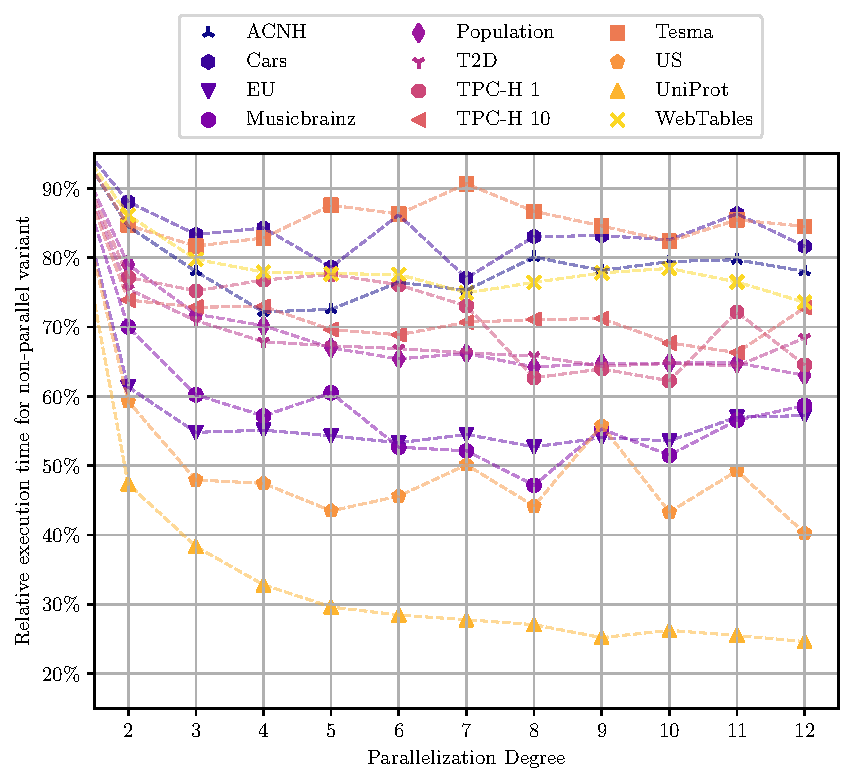
\includegraphics[width=0.475\textwidth]{figures/spider_parallel.pdf}
    \caption{Parallelization effectiveness for \textit{pSPIDER} over various datasets.}
    \label{fig:parallel_spider}
\end{figure}